
\section{Background \& Problem}

All Open Container Initiative compliant containers, including Kubernetes,
enforce CPU reservations using \cgroups{}' weight
interface~\cite{container-isolation-article}, as do VM frameworks, including
Firecracker and libvirt~\cite{firecracker-cgroups,libvirt-cgroups}. 

\begin{figure}[t]
    \centering
    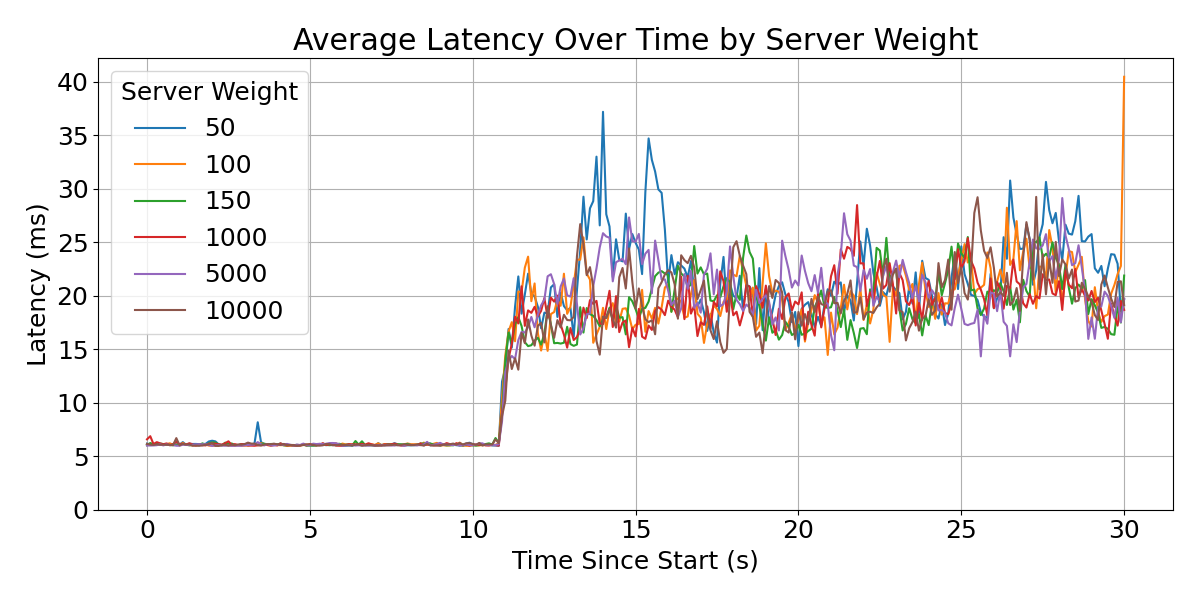
\includegraphics[width=0.9\columnwidth]{graphs/srv-bg-weight-cmp-low.png}
    \caption{ the weight of the server has little impact on how much the
    weight 1 BE task interferes }\label{fig:srv-bg-weight-cmp}
\end{figure}
% the weight of the server has little impact on how much the
%     weight 1 BE task interferes


A simplified experiment shows \cgroups{} weights are unable to enforce
reservations. We run a simple CPU-bound server sharing 4 cores with an image
resize job, each in their own group. \cgroups{} supports weights in the range
[1,10000]; \autoref{fig:srv-bg-weight-cmp} shows running the server with any
weight above 50 does not change the latency impact of the BE.

Visualizing the trace using schedviz~\cite{schedviz-tool} shows us this latency
impact happens because for up to 10s of milliseconds, one core runs a BE thread
(its own runqueue is otherwise empty), while server threads are queued on the
other cores.

This happens because weights are only enforced within per-CPU runqueues. Load
balancing eventually remedies imbalances, but runs less frequently than
scheduling. For workloads with request processing times in the millisecond
range, waiting for the load balancer affects processing times.

In order to globally enforce weights, each scheduling decision would require a
search of all runqueues for potentially higher-weight processes, which is too
costly. 




